\documentclass[letterpaper,12pt]{article}
\newcommand{\forceindent}{\leavevmode{\parindent=1.25em\indent}}

\usepackage{indentfirst, setspace, amssymb,amsmath,pdfpages,graphicx,float,soul,wrapfig}
\begin{document}
\doublespacing
\title{Cellular Automata on Regular Tilings of Hyperbolic 2-space}
\author{Michael Whalen}
\date{April 18, 2018}
\maketitle
\setlength{\parindent}{4em}

\section*{Introduction}

When I started this project, I really didn't have a good idea of its scope nor what I'd encounter along the way. I chose to do this project because I was vaguely familiar with hyperbolic tilings and thought they were fascinating, that they'd be a neat playground for cellular automata. I ended up spending the first half of the semester largely just reading textbooks and math journals to learn how to actually construct the geometric objects I was after. Throughout that whole time I was unsure that I'd actually be able to complete the project and even had another project idea as backup. A couple months in, though, everything seemed to finally click and the code started flowing like water. I ended up switching to Python rather than C++ because I found that most of my time was being spent struggling with quirks of the language and issues with Qt's bindings specific to C++. Python simplified the process while preserving the benefit that I can port the code back to C++ relatively easily.

The objective of my work is to create a platform where a user can create and explore cellular automata on regular tilings of hyperbolic space with minimal concern of the mathematical machinery.
I'll begin by describing the gist of the mathematics behind hyperbolic space, followed by a brief description of cellular automata and its relevance. Finally, I'll discuss my software implementation of these concepts.

\section*{Hyperbolic Geometry}

At the most basic level, \textbf{Hyperbolic Geometry} is exactly like the normal Euclidean geometry we're used to, with one twist: with Euclidean geometry, given a line and a point, there is only one other line through that point that is parallel to the given line. In hyperbolic space, we let there be an infinite amount. This one allowance gives way to a ton of interesting behaviors and can be modeled in a multitude of ways. For my purposes, I chose to use what's known as the Poincare model as it has a significant amount of research in it and was relatively simple to learn more about. In essence, the Poincare model is represented by a disk, wherein "lines" are defined to be arcs of Euclidean circles orthogonal to the disk.

Like Euclidean geometry, in hyperbolic geometry we can examine polygons. Moreover, we can create a \textbf{tiling} of the space using polygons of many kinds, i.e., the space is filled by interlocking, identical shapes. This project concerns itself only with regular polygons, but irregular polygons could be an interesting thing to explore as well. \textbf{Regular polygons} are shapes whose angle measures are uniform, like squares and pentagons in Euclidean space. The real restriction of Euclidean space however is that there are only three tilings of regular polygons: equilateral triangles, squares, and hexagons. Nothing else works as there will either be overlap of polygons or empty space. This is where the value of hyperbolic space comes into play: there exists an infinite number of regular polygons that tile the hyperbolic plane.

\section*{Describing Tilings}

Since there are so many tilings, I needed a simple and programmatic way of referring to individual tilings. This was done using a \textbf{Schl{\"a}fli Symbol}, notated as $\{p, q\}$, where $p$ denotes the number of sides on the polygon and $q$ denotes the number of polygons adjacent to any given vertex. For example, in Euclidean space we can represent the square tiling as \{4, 4\} since squares (four sides) meet four at each vertex. The other two possible tilings of Euclidean space are $\{3, 6\}$ (equilateral triangles) and $\{6, 3\}$ (hexagons). This symbol also provides a simple way for checking if a tiling is valid in hyperbolic space:
\begin{gather*}
\theta=1/p + 1/q
\end{gather*}
When $\theta<1/2$ the tiling is elliptic; when $\theta=1/2$ it's Euclidean; when $\theta>1/2$ it's hyperbolic.  These symbols lend themselves to a highly simplified software implementation of tilings.

\section*{Constructing Tilings}

So we know what a tiling is, but how do we make one? It's actually a question with a surprisingly simple solution, yet it took me a couple of months to realize it through extensive reading. We can construct hyperbolic tilings in exactly the same way that we might in Euclidean space: start with a polygon, reflect it about each of its sides, and repeat for these new polygons. The only real difference with hyperbolic space is the method of reflection. Because the sides of the polygon are sections of circles, reflecting a point about a side is the same as performing a Euclidean inversion about the corresponding circle.

\begin{wrapfigure}{r}{0.25\textwidth}
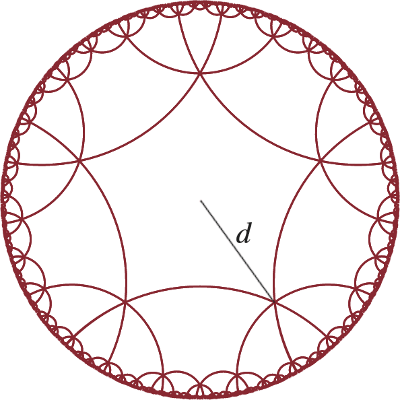
\includegraphics[width=0.25\textwidth]{../media/tilingDistance.png}
\end{wrapfigure}

The center polygon can by found by determining one value: the distance between the origin of the disk and one of its vertices. This distance $d$ is then used to find the first vertex of the polygon, which can be anywhere on the circle concentric with the disk and of radius $d$.  The remaining vertices can then be found by rotating this first vertex about the origin at $\frac{\pi}{p}$ intervals. The inital distance $d$ is calculated from the $p$ and $q$ values which specify the tiling:
\begin{gather*}
d = r\sqrt{\frac{cos(\frac{\pi}{p} + \frac{\pi}{q})}{cos(\frac{\pi}{p} - \frac{\pi}{q})}}
\end{gather*}

Then, the arcs between these vertices are constructed by first generating the Euclidean circles that constitute them. For example, for two vertices $A$ and $B$, generate a third point $C$ outside of the disk by inverting either A or B about the disk. The perpendicular bisectors $l$ and $m$ for the segments $AB$ and $BC$ respectively will intersect at a point $D$, which will be the center for the desired circle. Then it's trivial to construct the arc between A and B.

To create a tile adjacent to the center polygon, reflect all the vertices of the polygon about the common side by performing a Euclidean inversion of each vertex about the circle that makes up that side. This makes the vertices for the adjacent polygon and the process for generating its sides is a repetition of the process for the center polygon.

\section*{Cellular Automata}

Ultimately, the goal here is to use these fancy hyperbolic tilings as a tool for representing cellular automata. In a nutshell, these are sets of rules that govern the states of cells in some kind of tiling, where each timestep evaluates each tile and determines its next state based on the current states of itself and its neighbors. Typically these are represented on square grids (\{4,4\}) and "neighbors" of a tile are the eight tiles that surround it. Interesting behaviors may arise when we allow tiles to be strange, non-euclidean polygons. The software I've created is essentially just a platform for creating and exploring these automata in detail with a great amount of customization and interactivity.

As examples, I've created two automata that can operate on any tiling (though some tilings are more interesting than others): a version of John Conway's Game of Life and WireWorld. The game of life is rough around the edges and needs tweaking, but it a simple example with two states and basic rules for whether a tile lives or dies, depending on the number of live tiles next to it. Wireworld provides for a more interesting experience, where yellow tiles are a sort of "wire" and electrons, represented by a blue head and red tail, can travel along these wires. On some tilings this can create pulse generators of different intervals as well as basic logic gates.


\section*{Software Implementation}

The general structure of the program follows a Model-View-Controller pattern; however, due to the fact that a tiling's visual appearance is intimately connected with the software model, I had to combine the Model and View components into one class: PoincareViewModel. This class is the workhorse of the program, responsible for constructing and painting the tiling. It requires only three parameters to create the tiling: $p$ (sideCount), $q$ (adjacencyCount), and the maximum render depth, a limit on the number of consecutive reflections. See Figure 1 on page 9 to see how the classes are arranged for the program.

The tiling itself is a list of Tile objects, each of which is responsible for drawing itself and generating its QRegion, a Qt representation of the area the tile covers. Each Tile holds onto a list of neighbor Tiles and a list of Edge objects, where each Edge is responsible for performing the actual reflections of points/tiles. The tiling process is largely self-contained and can be interchanged with any other viewmodel class; for instance, a simple class to represent a Euclidean square tiling could be plugged into the rest of the program and function fine, so long as it implements the methods of the current viewmodel.

The PoincareViewModel is managed by a CellularController, which is essentially the brains of the program. It manages the interface next to the view and communicates with the viewmodel to make changes to it. Through the controller, the user can specify the sidecount/adjacencycount to create different tilings in addition to the render depth. See Figures 2 \& 3 on page 10 for examples of how the UI looks.

It also holds onto an Automaton object, which is responsible for performing the actual state changes on a given set of tiles. Subclassing Automaton is simple, with the only requirements being a list of states (QColors) and the nextGeneration() method. 

Finally, the MainWindow class has the responsibility of creating the PoincareViewModel, creating the CellularController on that viewmodel, and displaying them next to one another in the right proportion.

\section*{Conclusion}

At this point, I'm really satisfied with how the project turned out. I got all the major features that I was after and built it in such a way that adding more in the future shouldn't be too much of a hassle. By far, the largest problem I encountered was the issue of uniquely identifying tiles. The patchwork solution I have now is to index tiles by their hyperbolic centers as ordered pairs. This causes issues towards the outer rim when tiles get very small and the precision error of Python causes some tiles to be mistaken for others. This leads to some tiles being drawn more than once which is just unnecessary computation. The real solution to this is to identify tiles by the reflections needed to get from the center tile to it, using a bit of group theory. Then the actual comparison of generators would be done with the Knuth-Bendix completion algorithm, which works regardless of how small the tiles end up being. I hope that I can eventually implement this in the future, as well as the other features that I wasn't quite able to find time for. I'd also like to try using OpenGL to render the tilings since it's more optimized than Qt's QPainter. 

I learned a ton through this experience and it really felt like I was able to combine the subjects from most of my CS courses in one place, while also being able to incorporate some of my math courses. This is a project that I'll keep plugging away at on the side for a while since I see a lot of potential in it.\\

\section*{Figures}
\begin{figure}[H]
\hspace{-10em}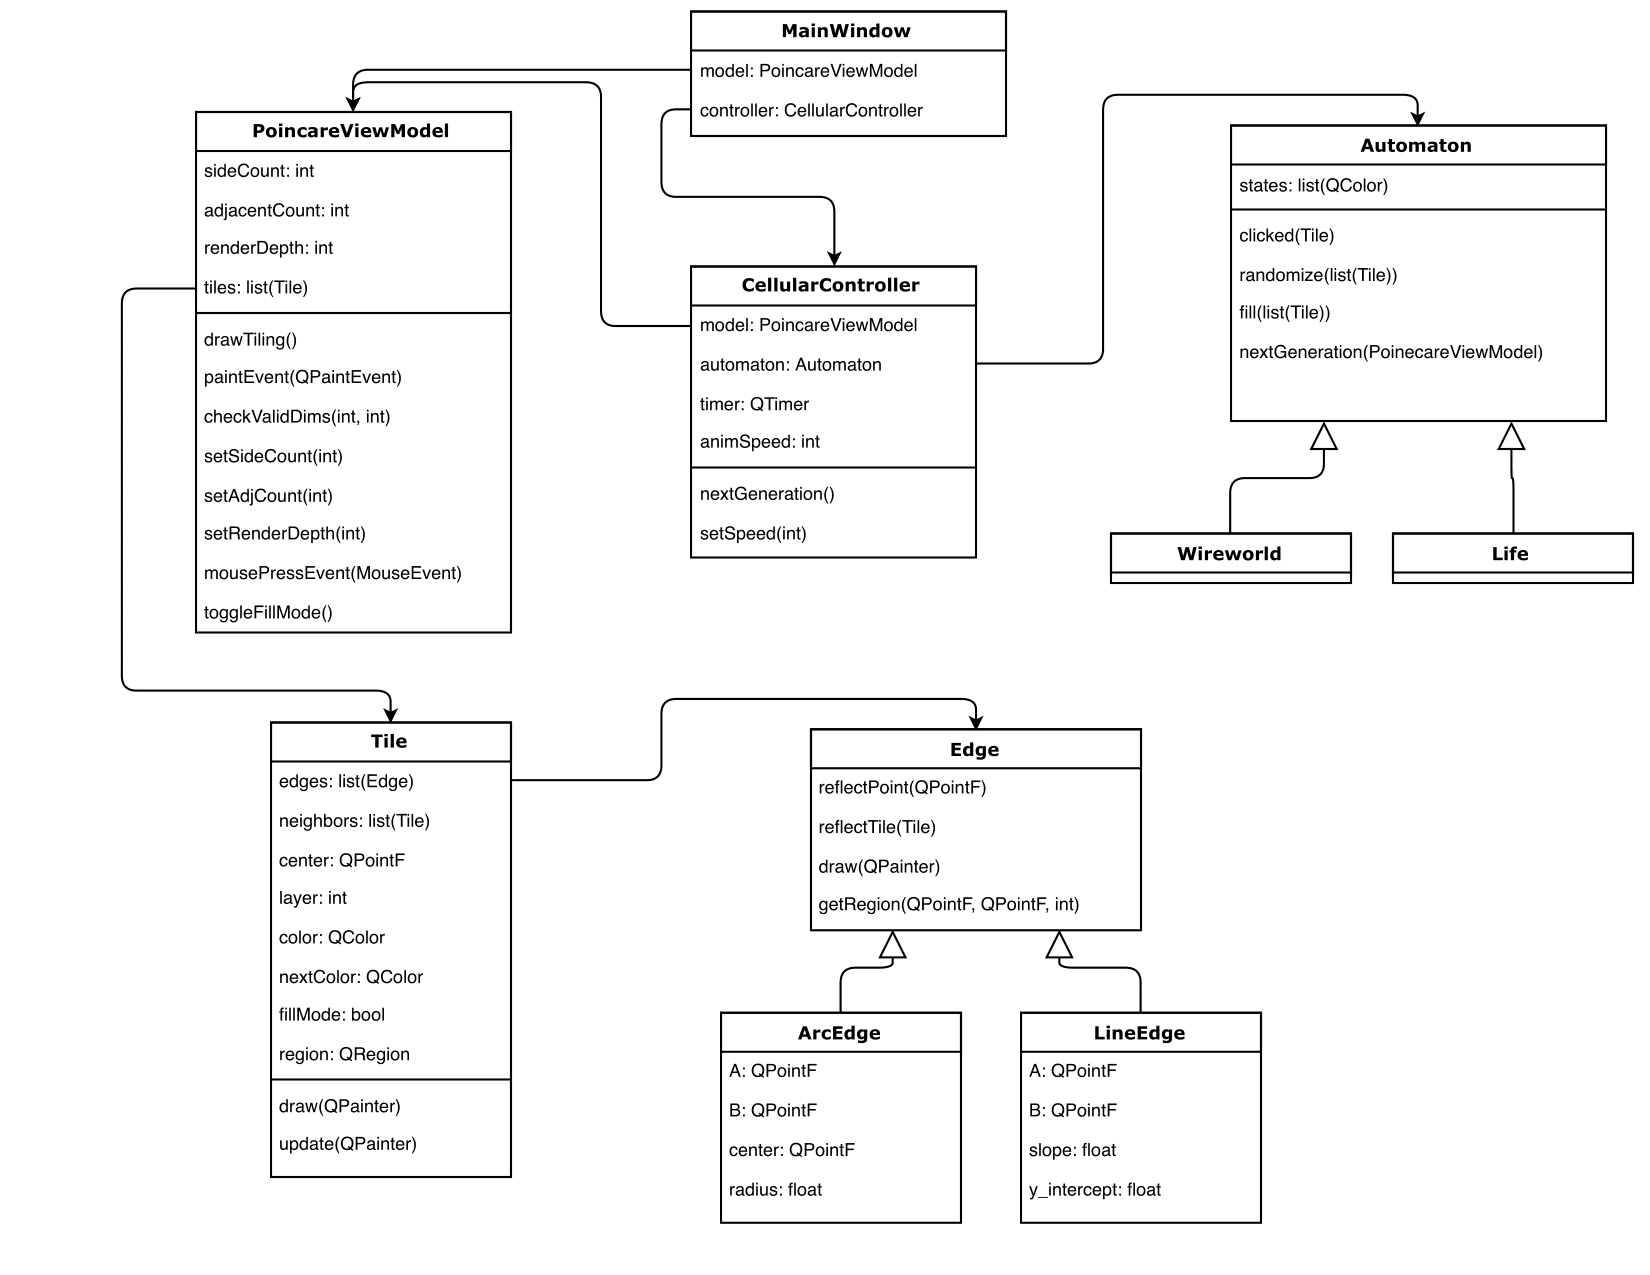
\includegraphics[width=\paperwidth]{../media/class_diagram.png}
\caption{Diagram of the classes created in the project.}
\centering
\end{figure}

\begin{figure}[H]
\vspace{-5em}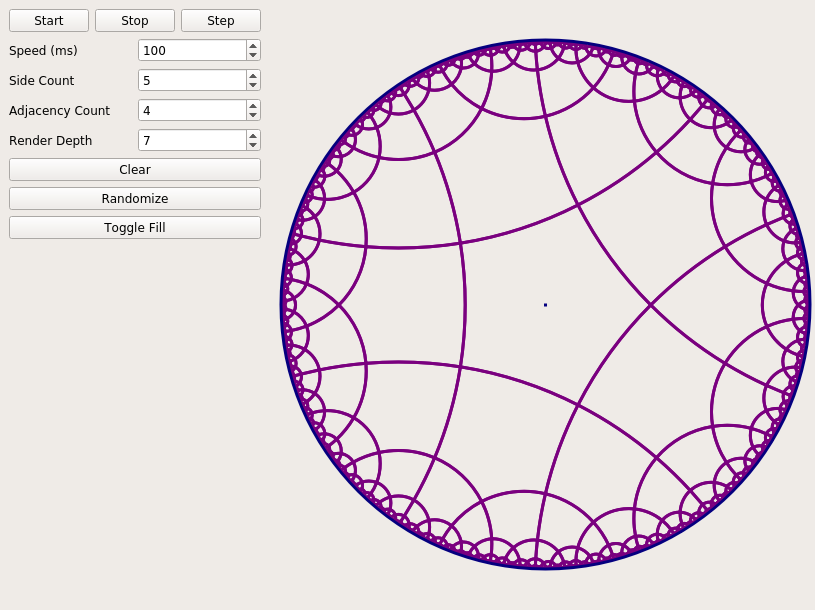
\includegraphics[width=29em]{../media/ui1.png}
\caption{The UI displaying a \{5,4\} tiling and no fill.}
\centering
\end{figure}

\begin{figure}[H]
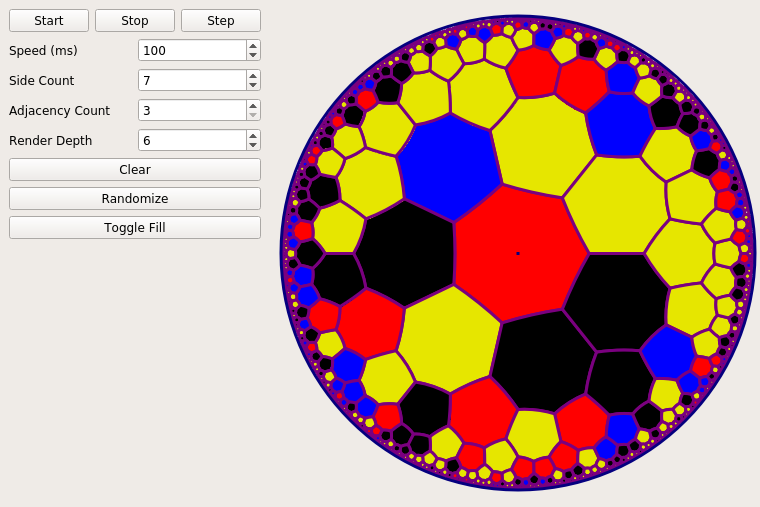
\includegraphics[width=29em]{../media/ui2.png}
\caption{The UI displaying a \{7,3\} tiling and wireworld fill.}
\centering
\end{figure}


\section*{Completed Points}

\footnotesize
	\hspace{-5em}
	\begin{tabular}{ | l | r | }
	    \hline
	    \textbf{Feature} & \textbf{Point Value} \\ \hline
	    \hl{Hyperbolic tilings of a single polygon} & 20 \\ \hline
	    \hl{Support arbitrarily many polygon types} & 20 \\ \hline
	    \hl{Color in the tilings according to an automaton} & 20 \\ \hline
	    \hl{Animate changes in state} & 10 \\ \hline
	    \hl{Supports multiple sets of rules} & 5 \\ \hline
		\hl{Supports an arbitrary amount of rulesets} & 10 \\ \hline
		\hl{Supports more than two states} & 5 \\ \hline
		\hl{Users can interactively change the state of cell by clicking} & 10 \\ \hline
		\hl{User selects cell dimensions} & 5 \\ \hline
		User inputs rulesets & 5 \\ \hline
		User inputs possible states & 3 \\ \hline
		User selects color of states & 3 \\ \hline
		\hl{User selects speed of animation} & 1 \\ \hline
		\hl{Start/stop animation} & 1 \\ \hline
		\hl{Step one generation at a time} & 1 \\ \hline
		Can save/load states and rules & 5 \\ \hline
		Can zoom in & 5 \\ \hline
		Zoom without losing resolution & 10 \\ \hline
		Can rotate view & 10 \\ \hline
		\textbf{Total Possible:} & \textbf{149} \\ \hline
		\textbf{Total Earned:} & \textbf{113} \\ \hline
	\end{tabular}
\quad
\footnotesize
\begin{tabular}{ | l | r | }
    \hline
    \textbf{Point Range} & \textbf{Grade} \\ \hline
    100+ & A \\ \hline
    85 - 99 & B \\ \hline
    70 - 84 & C \\ \hline
    50 - 69 & D \\ \hline
    Below 50 & F \\ \hline

 \end{tabular}
\end{document}